\documentclass{VUMIFInfKursinis}
\usepackage{algorithmicx}
\usepackage{algorithm}
\usepackage{algpseudocode}
\usepackage{amsfonts}
\usepackage{amsmath}
\usepackage{bm}
\usepackage{color}
\usepackage{graphicx}
% \usepackage{hyperref}  % Nuorodų aktyvavimas
\usepackage{url}
\usepackage{subcaption}	% package for subfigures
\usepackage{tabularx}
\usepackage{pythonhighlight}

% Titulinio aprašas
\university{Vilniaus universitetas}
\faculty{Matematikos ir informatikos fakultetas}
\institute{Informatikos institutas}  % Užkomentavus šią eilutę - institutas neįtraukiamas į titulinį
\department{Informatikos katedra}
\papertype{Kursinis darbo projektas}
% Nenurodytas vienas arba keli iš būtinų atributų: kalba, raktiniai žodžiai, santrauka.
\title{Automatizuotas kriptovaliutų prekybos robotas}
\titleineng{Automated cryptocurrency trading bot}
\status{4 kurso 1 grupės studentas}
\author{Matas Kaminskas}
\supervisor{J. Asist., Dr. Igor Katin}
\date{Vilnius \\ \the\year}

% Nustatymai
% \setmainfont{Palemonas}   % Pakeisti teksto šriftą į Palemonas (turi būti įdiegtas sistemoje)
\bibliography{bibliografija} 

\begin{document}
\maketitle

\tableofcontents

% Įvade apibūdinamas darbo tikslas, temos aktualumas ir siekiami rezultatai. 
\sectionnonum{Įvadas}
% could be better, say something about novel nature of cryptocurrency
Pasaulis vis labiau modernėja, technologijos tampa vis išmanesnės ir našesnės, nei bet kada anksčiau. Šiais laikais turime kontraversiškai pagarsėjusią
kriptovaliutų rinką, kuri yra kaip skaidresnė atsvara standartinei akcijų biržai. Po 2007-2008 metų įvykusios finansų krizės,
visai neužilgo - \cite{nakamoto2008bitcoin} 2008 metais, atsirado pirmoji kriptovaliuta - Bitcoin. Tai yra decentralizuotą ir nepriklausoma elektroninę valiutą, paremta
blokų grandinės technologija. Dabartiniais apskaičiavimais šios rinkos bendra vertė viršija 800 milijardų JAV dolerių \cite{CoinMarketCap},
nors kiek daugiau nei prieš metus ši vertė buvo dvigubai didesnė - 1.6 trilijonų JAV dolerių, o tarp 2018 ir 2020 metų vertė daugmaž buvo stabili - apie 100 milijardų JAV dolerių.
Šie duomenys dar kartą pabrėžia kriptovaliutų rinkos nepastovumą, bei ženkliai padidėjusi susidomėjimą, populiarumą visuomenėje.    


Pagrindinis skirtumas tarp kriptovaliutų rinkos ir tradicines akcijų biržos yra jog mainai vyksta 24 valandas per parą. Akcijų biržoje yra nustatytos pagrindinės darbo valandos,
jos dažniausiai yra tokios pat kaip vietos darbo valandos ir pagrindiniai mainai vyksta šiomis valandomis, todėl stebėti tendencijas ir realizuoti strategijas yra įmanomas darbas asmeniui.
Kai rinka yra prieinama visa parą dirbant be sustojimo yra nepraktiška, bei neįmanoma stebėti ir atlikti prasmingus mainus rinkoje. Atsiranda puiki terpė automatizuoti šį 
procesą - įdarbinti automatizuotą prekybos robotą, kuris gebėtų analizuoti rinkos duomenis ir prognozuoti tolimesnė rinkos eigą.


Pratęsiant kursinio darbo temą, šio kursinio darbo projekto tikslas yra sukurti automatizuotą kriptovaliutų prekybos robotą. 
Darbe pritaikomas autoregresinių modelių veikimas, pagal kuriuos robotas galės remtis atliekant kriptovaliutų rinkos mainus. 

Tikslui įgyvendinti keliami uždaviniai:
\begin{itemize}
  \item mokslinės literatūros analizė,
  \item autoregresinių modelių analizė ir pritaikymas,
  \item sukurti robotą gebanti remtis ištirtų modelių prognozėmis,
  \item paleisti robotą prekiauti testiniame tinkle,
  \item ištirti gautus rezultatus.
\end{itemize}


%Pagrindinėje tiriamojoje dalyje aptariama ir pagrindžiama tyrimo metodika;
%pagal atitinkamas darbo dalis, nuosekliai, panaudojant lyginamosios analizės,
%klasifikacijos, sisteminimo metodus bei apibendrinimus, dėstoma sukaupta ir išanalizuota medžiaga.
\section{Pagrindinė tiriamoji dalis}
% citation about impact of bitcoin on other coins? Explain mining (savoka)?
% koks tinklas?
Pagrindinė ir pirmoji kriptovaliuta - Bitcoin. Nors pirmieji 50 BTC buvo "iškasti" 2009 metų pradžioje, Bitcoin susilaukė didesnio dėmesio
tik 2013 metais\cite{macdonell2014popping}. Ši kriptovaliuta buvo laikoma ateities valiuta dėl savo naujoviškumo ir decentralizavimo, bet susilaukdavo ir 
neigiamų atsilipiemų dėl atsiskaitymo nelegaliuose prekybos vietuose internete. 
Vienas pirmųjų ir itin didelės apyvartos sulaukęs nelegalių prekių tinklalapis "Silkroad" atsiskaitymui už prekes naudojo Bitcoin.
Didelė apyvarta skatino bitcoin augimą, susidomėjimą ir kitų kriptovaliutų progresą.
% Source on correlation
Stebint kriptovaliutų rinką matoma koreliacija tarp Bitcoin kainos ir visų kitų kriptovaliutų kainos, taip dar kartą pabrėžiama, jog ši valiuta yra pagrindinė rinkoje.
Kyla bitcoin kaina - kyla kitų valiutų kaina, krenta bitcoin kaina - krenta kitų valiutų kaina. Retesniais atvejais kriptovaliutos sparčiau keičia kainą dėl 
pažangaus vystymosi ar dėl esančių problemų. 
% SOL auga labai? XRP freeze del teismo? ADA kyla nes pazangi, nors btc stabilus? ir kiti E.g. nezinu ar reikia čia šitą plėstis

% source on limited sources?
Dauguma kriptovaliutų yra riboto kiekio, tad jeigu prekybos robotas uždirba konkrečios kriptovaliutos mažai, jų kainą gali keleriopai išaugti 
tikrų valiutų atžvilgiu, todėl į kriptovaliutą galima žiūrėti ir kaip į investiciją. 2018 metais, nepaisant to, kad kriptovaliuta buvo galima 
atsiskaityti už paslaugas ar prekes, populiauriausia paskirtis buvo investicija. Viena iš priežaščių - tuo metu kaina buvo pakilus nenuspėjamai
aukštai\cite{garg2018autoregressive}. Akcijų birža, rinka naudojama investiciniais tikslais, jau kurį laiką yra analizuojama dėl savo finansinės
naudos ir sudėtingumo. Šios rinkos turi panašumų, todėl galima tirti akcijų biržos analizė literatūroje.

% Citation needed on cryptocurrency block chain, anonimty and everything else!
Šiais laikais vis daugiau žmonių naudojasi technologijomis ir nori nepriklausomybės nuo institucijų išleidžiamų ir manipuliuojami valiutų, infliacijos ir kitų dalykų, 
kurie mažina finansinių instituticijų pasitikėjimą. Kriptovaliutos yra paremtos blokų grandinės technologija, todėl daugelis jų yra decentralizuoti tinklai. 
Visa blokų informacija yra viešai prieinama publikai, puikiai žinoma tarp kokių šalių vyksta sandoriai, taip suteikiamas skaidresnis ir patikimesnis būdas publikai
turėti savo nepriklausomą rinką. Ypatingas kriptovaliutų bruožas yra tas, kad jų paprastai neišleidžia jokia centrinė institucija, todėl teoriškai jos nėra 
apsaugotos nuo vyriausybės kišimosi. Ankščiau minėtos savybės suteikia anonimiškumo, todėl tai sudaro palankias sąlygas klestėti sukčiavimo atvejams, 
"pump-and-dump" ar "ponzi" schemoms. Dažniausiai sutinkama yra "pump-and-dump" schema, kuri apibūdina procesą, kai valiutos paklausa yra iš anksto
apgalvotai ir trumpam padidinima, taip pakeliant jos kainą, vėliau, kai kainą yra pasiekusi tinkamą tašką, organizatoriai, staigiai parduoda savo
turimą kiekį, taip pasipelnydami\cite{xu2019anatomy}.

%social media influence?
Pagrindinis tyrimas šiame darbe yra tinkamiausio auto regresinio modelio parinkimas automatizuotam robotui lošėjui. Lošimo procesas tam tikrą laiką gali būti atliekamas žmogaus, 
stebėti besikeičiančias kainas ir atitinkamai elgtis, tačiau toks darbas yra monotoniškas ir atsiranda natūrali terpė jį automatizuoti. Automatizavimui
reikia taikyti pasirinktą strategiją, kuri spręstų kada yra tinkamas metas įsigyti kriptovaliutą, o kada parduoti, bet pirmiausia reikalingas tinkamas prognozavimo modelis.
Auto regresiniai modeliai taikomi laiko eilutėmis yra paplitę statistikoje norint prognozuoti tendenciją ateityje. Modelio prognozės tikslumui bei tinkamumui palyginti 
bus naudojama santykinė ir absoliuti klaidos.

\subsection{Darbinė aplinka}
Šiam robotui ir statistiniams modeliams teks naudotis jau sukurtais įrankiais, kurie palengvins darbą. Naudojama Python programavimo kalbą, 
kadangi ši kalba turi patogų API su dauguma kriptovaliutų rinkų ir patogias bibliotekas autoregresyviems modeliams bei kitiems reikalingiems API.

\subsubsection{Python}
Python yra aukšto lygio programavimo kalba. Joje galima sutikti ne viena programavimo paradigmą: procedurinę, objektinę ir netgi funkcinę.
Ši kalba suteikia patogu abstrakcijos lygį šiai užduočiai - automatizuoti robotą lošėją ir panaudoti AR modelius.
Šiais laikais python yra viena populiariausių kalbų pasaulyje, dėl savo paprastumo ir paprasto naudojomo naujam vartotojui, bet tikrai yra daugybę savybių
kuriomis prireiktų ne vienus metus suprasti ir prasmingai naudoti programuojant. Dėl šios kalbos privalumų dauguma egzistuojančių API
bibliotekų palaiko Python programavimo kalbą.


\subsubsubsection{Python-binance API}
Šiame darbe naudojama "python-binance" API. Šis API yra "Wrapper" oficialiam Binance API - binance-connector-python. 
Oficialus API yra labai paprastas ir lengvasvoris, todėl didelio patogumo nėra, tik paprasčiausios užklausos,
kurias visvien reikėtų apdoroti, labai padeda padaryti šis wrapper API - python-binance.

\subsubsection{Binance}
Binance yra didžiausia kriptovaliutų birža pagal prekybos apimtį, turinti itin didelį valiutų pasiulą ir patogiai prieinamus duomenis. Ši birža taip pat
suteikia galimybė "lošti" kriptovaliutomis testiniame tinkle. Tinklo paskirtis yra lengvai nuspėjama iš pavadinimo, jame galima atlikti tuos pačius 
% issiplesti ir papasakoti apie rinkoje galimus atlikti veiksmus, LIMIT BUY, LIMIT SELL ir t.t.
veiksmus kaip realioje rinkoje, tik naudojama netikra valiuta kuri tikros vertės neturi.

% kas yra SPOT market parašyti? https://academy.binance.com/en/articles/a-complete-guide-to-cryptocurrency-trading-for-beginners
\subsubsubsection{Binance Spot Test Network}
Testinis tinklas yra beveik identiškas tikrajam "Binance" tinklui, kainos yra vienodos kaip ir pagrindiniame tinkle ar pasaulyje, todėl galima analizuoti 
seniausius rinkos duomenis ir juos taikyti reikiame modelyje. Testinis tinklas nėra toks populiarus, tad jame yra ženkliai mažiau prekiaujančių žmonių. 
Testiniame tinkle pąskyra sukuriama naudojant "Github" prisijungimą. Kiekvienas naujas vartotojas turi pradinį balansą susidendantį iš kriptovaliutų
matomų 1 lentelėje.

\begin{table}[H]\footnotesize
  % tablesgenerator.com - converts calculators (e.g. excel) tables to LaTeX
  \centering
  \caption{Pradinis likutis}
  {\begin{tabular}{|l|c|} \hline
      Kriptovaliuta & Kiekis  \\
      \hline
      BNB           & 1,000   \\
      BTC           & 1       \\
      BUSD          & 10,000  \\
      ETH           & 100     \\
      LTC           & 500     \\
      TRX           & 500,000 \\
      USDT          & 10,000  \\
      XRP           & 50,000  \\
      \hline 
    \end{tabular}}
\end{table}

Šiuo likučiu galima elgtis kaip norima. Pradinis likutis yra pakankamas atlikti prasmingoms transakcijomis testiniame tinkle. Reikėtų pabrėžti, jog testinis
tinklas kas mėnesį laiko yra iš naujo nustatomas ir visas turimas likutis yra konvertuojamas atgal į pradinį likutį, išvalant ankščiau buvusį balansą, tad jeigu
nepavyko praturtėti prekiaujant kriptovaliutomis, vėl įgaunama proga pradėti prekyba, na o sėkmingu atveju visas pelnas yra ištrinamas ir reikia vėl pradėti
nuo nulio.

% interpolation vs extrapolation?
\section{Laiko eilučių analizė}
"Visi modeliai yra klaidingi. Kai kurie modeliai yra naudingi" (angl. "All models are wrong. Some models are useful") - citata priskiriama George Box, kurios
reikėtų nepamiršti analizuojant laiko eilutes. Šis analizės būdas bando pastebėti pasikartojančius modelius bėgant laikui, jog būtų galima atlikti kuo tikslesnes
prognozes apie ateitį. 
Dažnu atveju tai yra vienas ar keli izoliuoti kintamieji, kurie yra stebimi nustatytą laiko tarpą ar surenkant jų istorinius duomenis. Laiko eilučių duomenų 
rinkimo ir analizavimo pavyzdžiai: sekamas paciento širdies pulsas, prekyboje sandelio prekių kieko priežiūra, konkrečios akcijos kainos prognozavimas akcijų biržoje. 
Laiko eilučių analizės vienas iš tikslų yra nuspėti kaip kinta reikšmė bėgant laikui, tai ir yra ko prireiks norint prognozuoti kriptovaliutų kainą šiam robotui. 
Kriptovaliutų kainų duomenys, taip pat yra laiko eilutė, nes kaina yra sekama bėgant laikui, tačiau dažniausiu atveju tai nėra stacionari laiko eilutė.
Reikia pabrėžti, kad toks analizės būdas tik bando nuspėti koks yra labiausiai tikėtinas rezultatas remiantis turimais duomeninimis ir naudojamu modeliu. 

\subsection {Laiko eilutės}
Laiko eilutė yra chronologiškai surikiuotas duomenų rinkinys. Laiko eilučiu analize analitkai gali pastebėti įvairias tendencijas ir taip prognozuoti reikšmes
ateityje bei geriau pasiruošti įvykiams. Laiko eilutė gali būti stacionari arba ne stacionari. Šiame darbe norint analizuoti turimus duomenis naudojant 
autoregresyvius modelius reikia turėti stacionarią laiko eilutę, jog būtų galima pritaikyti autoregresiniui modeliui. Tačiau kriptovaliutų kainą dažnu atveju yra
ne stacionari laiko eilutė, todėl prieš dirbant, reikia atitinkamai šiuos duomenis susitvarkyti arba analizuoti kitas eilutes.

\subsection {Laiko eilučių stacionarumas}
Stacionari laiko eilutė yra laikoma tokia eilutė, kurios statistinės savybės bėgant laikui nekinta \cite{nason2006stationary}. Tai reiškia, jog laiko eilutės vidurkis,
variacija ir kovariacija turi pastovias reikšmes. Stacionarios laiko eilutės yra lengviau analizuojamos, todėl autoregresyvieji modeliai yra pritaikyti dirbti su 
stacionariais duomenimis. Autoregresinių modelių taikymas nestacionariems duomenims gali suteikti nepatikimas prognozes ir prastesnius rezultatus. 
Prieš dirbant su duomenimis, juos galima pasiversti stacionariais, panaikinant sezoniškumus ar tendencijas imtyje.

\begin{figure}[H]
  \centering
  \begin{subfigure}{.5\textwidth}
    \centering
    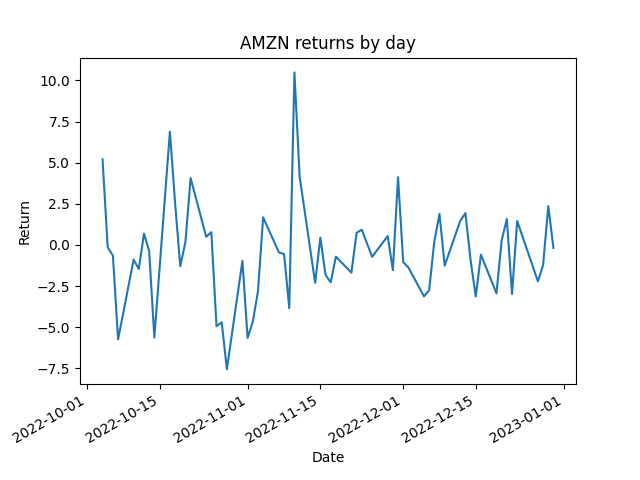
\includegraphics[width=.6\linewidth]{img/AMZN_daily_return.png}
    \caption{Stacionari laiko eilutė}
    \label{fig:sub1}
  \end{subfigure}%
  \begin{subfigure}{.5\textwidth}
    \centering
    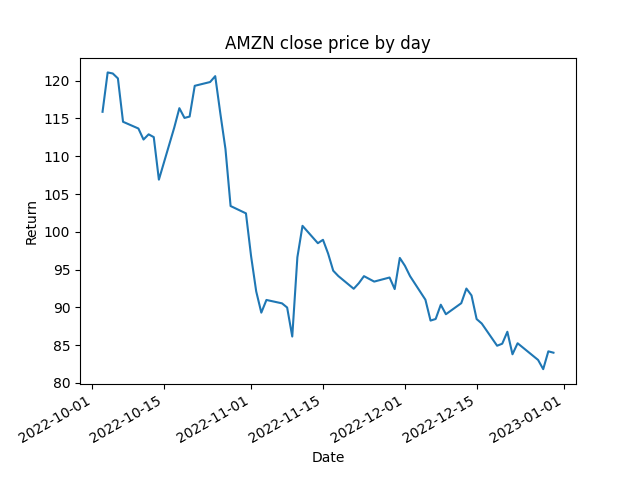
\includegraphics[width=.6\linewidth]{img/AMZN_daily_close.png}
    \caption{Nestacionari}
    \label{fig:sub2}
  \end{subfigure}
  \caption{Stacionari ir nestacionari laiko eilutė}
  \label{fig:test}
\end{figure}

Grafai parodantys skirtumą tarp stacionarios ir nestacionarios laiko eilutės. Grafuose naudojama "Amazon" kompanijos (NASDAQ: AMZN) akcijos duomenys gauti iš "Yahoo Finance" 
naudojant Python API\cite{yfinance}. Pirmajame (stacionariame) grafe yra pavaizduota kiekvienos dienos grąža investuojant į AMZN akciją trijų mėnesių laikotarpyje. 
Stacionarumas matomas ir vizualiai - vidurkis imtyje išlieka panašus, centruojasi ties 0, taip pat
% Variacija parodo kaip toli yra išsiskirste skaičiai imtyje, tai stacionariu atveju, nuo nulio atrodo visi panašų range turi. Variacija != standard deviation
% Kovariacija parodo kaip du kintamieji yra susije (teigiamai jei abu keičiasi vienodai arba negiamai jei keičaisi skirtinga kryptimi), čia svarbu kad ji išliktu vienoda (0 - nera rysio)
variacija ir kovariacija yra panašūs visuose taškuose. Antrame grafe yra pavaizduota tos pačios akcijos uždarymo kaina tokiame pat laikotarpyje. 
Nestacionarumas matomas ir vizualiai, kadangi yra akivaizdi tendencija žemyn. Šiuos teiginius patvirtina ir ADF testas. % Do I need to cite? 

% There are a few things you can try to improve the test:
% try using a different test for stationarity, such as the Kwiatkowski-Phillips-Schmidt-Shin (KPSS) test or the Phillips-Perron (PP) test.
% try differencing the data to remove any trend or seasonality. This can help to stabilize the variance of the data and make it more stationary.
% try applying a transformation to the data, such as taking the log of the data, to stabilize the variance and make the data more stationary.
% try using more data in the test. A larger sample size may provide more accurate results.
% try using a longer time period for the test. This can provide a more accurate assessment of stationarity, as it takes into account any long-term trends or seasonality in the data.
\subsection{ADF testas}
ADF (Angl. Augmented Dickey-Fuller) testas nustato ar laiko eilutė yra stacionari. Tai yra dažnai naudojamas įrankis analizuojant laiko eilutės ir jų algoritmais, kurie tikisi stacionarių 
duomenų\cite{chi2018stock}. Stacionariai laiko eilutėje privaloma atmesti nulinę hipotezę tam tikrame užtikrintumo intervale. 
Jeigu ADF testo absoliuti statistinė vertė yra daugiau už kritinę vertę, nulinę hipotezę yra atmetama ir ši laiko eilutė yra stacionari.
pritaikius ADF testą{\cite{seabold2010statsmodels}} AMZN akcijų duomenims (\textbf{1 pav.}) gauti rezultatai:

% p reiksme, alfa reiksmingumo lygis
\begin{tabularx}{\linewidth}{|X|X|X|X|X|X|}
  \hline
  \textbf{Time Series} & \textbf{ADF Statistic} & \textbf{p-value} & \textbf{1\% Critical Value} & \textbf{5\% Critical Value} & \textbf{10\% Critical Value} \\ \hline
  Daily Returns        & -7.087                 & 0.000            & -3.542                      & -2.910                      & -2.593                       \\ \hline
  Daily Close Price    & -1.640                 & 0.461            & -3.542                      & -2.910                      & -2.593                       \\ \hline
\end{tabularx}

\vspace{10pt}
Pagal šiuos rezultatus
\begin{itemize}
  \item ADF statistika yra skaičius, kuris lyginamas su kritinėmis vertėmis iš lentelės (skirtingais lygiais), kad būtų nuspręsta, ar atmesti ar priimti nulinę hipotezę apie stacionarumą.
  \item Pirmu atveju ADF statistika dienos grąžoms yra -7.087, kuri mažesnė, nei kritinė vertė -3.542 1\% lygyje. Todėl nulinė hipotezė yra atmesta ir laiko eilutė laikoma stacionari.
  \item Antru atveju ADF statistika dienos uždarymo kainoms yra -1.640, kuri yra nemažesnė, nei kritinė vertė -3.542 1\% lygyje. Todėl nulio hipotezė nėra atmesta ir laiko eilutė laikoma nestacionari.
\end{itemize}

\section{Autoregresiniai modeliai}
Vienas iš būdų analizuoti laiko eilutės yra autoregresija ir ją naudojantis modeliai. Egzistuoja ne vienas autoregresija naudojantis modelis. 
Populiarusi ir dažniausiai sutinkami modeliai yra ARMA(p, q) ir ARIMA(p, d, q).
Šie modeliai taip pat naudojasi anksčiau nepaminėtu MA modeliu kuris yra slankaus vidurkio modelis (angl. MA - moving average).
Taip pat yra SARIMA, SARFIMA ir kitų modelių, turinčių savo specifinius panaudjimo atvejus. 

\subsection{AR modelis}
AR (angl. autoregressive) modelis remiasi tik praeities duomenimis, kad nuspėti kintamojo reikšme ateityje, ieškoma ar pastebimas pasikartojantis
modelis, kuris padėtų tiksliau nuspėti dydį ateityje\cite{chi2018stock}. Šis modelis dar dažnai vadinamas ARp modeliu, nes naudojamas kintamasis "p", nusakantis kiek praeiteis reikšmių 
iš laiko periodo norima naudoti. Laikant, kad kintamasis X yra laiko eilutės kintamasis AR(p) modelio formulė gali atrodyti taip: 
\[X_{t} = \Phi _{1}X_{t-1}+\epsilon_{t} \]

%\cite{chi2018stock} naudojami AR, MA ir ARMA modelio formulėms
${X_t}$ - stacionari laiko eilutė, $\Phi$ - AR modelio koeficientas, P - AR modelio laipsnis, $ \epsilon_{t} $ - AR modelio paklaida.

\subsection {MA modelis}
Toliau tyrinėjami autoregresyvieji modeliai susideda iš dar vienos dalies - Slankaus vidurkio - MA (angl. Moving average). Slenkančio vidurkio dabartinė
reikšmė tiesiškai priklauso nuo dabartines ir praeitų reikšmių. Žymėjimas MA(q) reiškia q laipsnio slenkamajį vidurkį, kurio formulę atrodo taip:  
\[X_{t} = \epsilon_{t} - \sum_{i=1}^{q}\theta_{i}  \epsilon_{t-i}\]

${X_t}$ - stacionari laiko eilutė, q - MA modelio laipsnis, ${\epsilon_t}$ - MA modelio paklaida.

\subsection {ARMA modelis}
ARMA (angl. autorogressive moving average) modelis yra autoregresyviaus ir slankaus vidurkio modelio junginys. Modelis dažnai žymimas
kaip ARMA(p, q), kur p yra AR laipsnis, o q yra MA laispnis. Pirmą kartą sujungtas 1938 mokslininko Herman Wold, jis pastebėjo jog ARMA modelis gal apimti 
dideles stacionarias laiko eilutes, kai yra tinkamai nurodytas p laipsnis ir q laipsnis\cite{makridakis1997arma}. Taip pat reikia pabrėžti, 
jog ARMA(0, q) = MA(q) ir ARMA(p, 0) = AR(p) Reiškia, jog Xt eilutė gali būti modeliuojama kaip kombinacija praeities $x_{t}$ reikšmių ir/arba praeities $e_{t}$ klaidų:
\[X_{t} = \phi_{1}x_{t-1} + \phi_{2}x_{t-2} + ... + \phi_{p}x_{t-p} + e_{t} - \theta_{1}e_{t-1} - \theta_{2}e_{t-2} - ... - \theta_{q}e_{t-q}\]


\subsection {ARIMA modelis}
ARIMA (angl. autoregressive integrated moving average) modelis yra paplitęs nuo 1970-ųjų iki šių dienų. Modelio pavadinimo šifravimas
pažodžiui: AR - Autoregresinis modelis, I - Integracija (Diferencijavimas), atsižvelgiama į duomenų tendenciją, MA - (Moving average) slankusis vidurkis.
AR ir MA yra atskiri modeliai, kurie gali būti naudojami paprastesnei laiko eilučiu analizei. Šio modelio privalumas, jog jis sujungia AR ir MA naudojimą kartu su
diferencijavimu, kuris suteikia galimybė giliau analizuoti laiko eilutes. Diferencijavimo dalis turimus duomenis padeda paversti į stacionarius, 
kurie yra reikalingi korektiškam modelio veikimui. Diferencijavimas vyksta baigtinį kartų skaičių, jog būtų pasiekta beveik-validi stacionari būseną. 
Kitais žodžiais ARIMA yra ekvivalentus ARMA modelis tiem patiems MA ir AR laipsniams \cite{hua2020bitcoin}. Taigi ARIMA modelis yra paremtas ARMA modeliu. 
Pagrindinis skirtumas tarp šių modelių yra tas, jog ARIMA konvertuoja nestacionarius duomenis į stacionarius prieš dirbant su jais. Modelio tipas yra 
klasifikuojamas kaip ARIMA(p,d,q), kur p - autoregresyvoji dalis, d - integravimo (diferencijavimo) dalis, q - slenkančio vidurkio dalis. Visos ARIMA modelio
reikšmės yra neneigiami sveikieji skaičiai \cite{mondal2014study}.

% Not sure about this
% dažniausiai negalima naudoti šiame kontekste
Dažniausiai yra 3 žingsniai naudoti ARIMA modelį:
\begin{enumerate}
  \item Duomenų surinkimas ir verifikavimas - tikriname ar gauti duomenys yra stacionarūs ir ieškome sezoniškumo.
  \item Diferencijavimas - vertimas laiko eilutę į stacionarią.
  \item Prognozavimas naudojant ARIMA modelį - dažniausias taikomas ARIMA modelis yra ARIMA(1,1,0)
\end{enumerate}

\subsection {SARIMA modelis}
SARIMA (angl. seasonal autoregressive integrated moving average) modelis yra ARIMA modelio išplėtimas turintis vieną papildomą savybę - sezoniškumą\cite{carl2020ethereum}. 
Pastebėjus, jog periodiškai kartojasi rezultatai laiko eilutėse, galima taikyti šį modelį. Geras ir paprastas pavyzdys, prekyba šventiniu laikotarpiu - kalėdos.
Prekybos centruose, tuo metu padidėja prekybą, tačiau kitą mėnesį ženkliai sumažėja. Spartus sumažėjimas nereiškia, jog prekybai yra didėlės problemos ir reikia pokyčių.
Tai dažniausiai yra žmonių poilsis nuo pirkinių po šventinio laikotarpio. šis modelis pastebi panašius sezoniškai atsitinkančius įvykius, juos atpažįsta ir pritaiko naudojant
ankščiau minėtą ARIMA modelį.

SARIMA galima išreikšti kaip ARIMA(p,d,q)(P,D,Q)[S], kur p,d,q standartiniai ARIMA modelio parametrai, o P - sezoniškumo autoregresivumo laipsnis,
D - sezoniškumo diferencijavimo laipsnis, Q - sezoniškumo slankiojo vidurkio laipsnis ir S - sezoniškumo ciklio ilgis. 

\section{Metodika}

Skyriuje aprašomi žingsniai, kurių buvo imtasi atliekant tyrimus ir analizę kuriant automatizuotą kriptovaliutų prekybos robotą. 
Tyrimo metu pagrindinis dėmesys buvo skiriamas tinkamų kriptovaliutų kainų analizės ir prognozavimo įrankiams ir metodams nustatyti bei skirtingų modelių veikimui įvertinti. 
Duomenys buvo renkami iš Binance testavimo tinklo naudojant python-binance API, o duomenims pritaikyti statistinės ir laiko eilučių analizės metodai. 
Kainų prognozavimui buvo naudojami autoregresyvūs modeliai, tokie kaip ARIMA ir SARIMA. 
Šio tyrimo išvados yra vienas iš pagrindų kuriant prekybos robotą.


\subsection{Modeliai}
Prognozavimui bus naudojami ARIMA ir SARIMA modelis. Kadangi kriptovaliutų kainų duomenys nėra stacionarūs, todėl naudojamas ARIMA modelis, kuris gali taikyti diferencijavimą.
ARIMA naudoja anksčiau minėtus AR ir MA modelius, bei pritaiko diferencijavimą, taip galėdamas dirbti ir su nestacionariais duomenimis. 
Jeigu laiko eilutė yra nestacionari ir bandoma naudoti AR, MA ir ARMA modelius, rezultatai galimai bus klaidingi arba netikslūs.
Taip pat naudojamas SARIMA modelis, nes jis yra ARIMA modelio pratęsimas tiriantis sezoniškumą laiko eilutėje, todėl dar bus patikrinama ar duomenyse egzistuoja sezoniškumas
galintis padėti prognozuoti.

% since network is test, used highest volatility pairs
\subsection{Duomenys}
Istoriniai duomenys "Candlesticks" surinkti iš Binance testavimo tinklo naudojant python-binance API. Kadangi testinis tinklas kiekvieną mėnesį automatiškai 
išvalo visus duomenis, imami 2023m. sausio 4d. duomenys savaitei į priekį, todėl verta paminėti, kad šie duomenys galioja tik tam tikrą laikotarpį. 
Kadangi tinklas yra testinis, jame prekiaujama nevisomis galimomis kriptovaliutų poromis. Iš viso yra 20 skirtingų porų tinkle. Pasirinkta tirti šias poras: 
i) BTC/BUSD, ii) LTC/BUSD, iii) XRP/BUSD.
Gaunamuose duomenyse yra daugiau informacijos bet bus naudojama tik datos ir `close' stulpelis, parodantis konkrečios kriptovaliutos uždarymo kainą tam tikru laiku. Tai yra paskutinė 
kaina, už kurią buvo prekiaujama tam tikru laikotarpiu, pavyzdžiui, valandą ar dieną. Uždarymo kaina yra svarbi, nes ji atspindi galutinę kainą, už kurią pirkėjai ir pardavėjai
sutarė prekiauti kriptovaliuta. Duomenys bus naudojami tokie kokie yra ir iškarto perduodami į modelius. Modeliui apmokyti naudojamas 90 procentų dumomenų rinkinio dydis.
Kitus 10\% bandoma prognozuoti po vieną reikšmę į priekį. Modeliui atlikus prognozė, jis yra iš naujo apmokomas pridėjus tikrąją sekančią vertę prie mokymo rinkinio ir
taip vėl yra prognozuojama kitą reikšmė, jau su naujai apmokytu modeliu.

% A detailed explanation of the model fitting process, including the specific parameters that you will be using for each of the AR models and any assumptions that you will be making.
\subsection{Modelių implementavimas}
Prognozuojant naudojamos ARIMA ir SARIMA pagalbinės bibliotekos\cite{seabold2010statsmodels} kuri aprašo šiuos modelius, 
bei euristins auto\_arima algoritmas\cite{pmdarima} padedantis nustatyti geriausius ARIMA ir SARIMA parametrus konkrečiam duomenų rinkiniui.
SARIMA modeliui sezoniškumo intervalas naudojamas 4 - bandoma pamatyti ar atsiranda sezoniškumas kiekvieną valandą, nes duomenų intervalas yra 15min.
Modelių vertinimui bus naudojama MSE ir MAPE paklaidos.

\subsection{Prognozavimas}

Kriptovaliutų kainų prognozavimo metodas naudoja anksčiau minėtus modelius ir Binance testinio tinklo duomenis. 
Žemiau matoma struktūrinę schemą, parodanti bendrą procesą, kurį sudaro keli pagrindiniai žingsniai. 
Pirmas žingsnis yra duomenų gavimas is binance API, bet jų gaunama daugiau negu reikia, todėl atsirenkami tik reikalingi duomenys, šis žingsnis yra
svarbus norint įsitikinti,kad duomenys yra paruošti analizei. Po to pasirenkame modelį (ARIMA/SARIMA).
Kitame žingsnyje yra gaunami geriausi parametrai konkrečiam duomenų rinkiniui ir modeliui, kad būtų optimalus veikimas. 
Tada taikome modelį treniruočių duomenims, kad apmokyti modelį tolimesniam prognozavimui. 
Po to modelis prognozuoja reikšmes ir jos yra saugomos, kad būtų galima palyginti su tikromis reikšmemis. Paskutinis žingsnis - palyginti gautus rezultatus
ir išsaugoti duomenis grafe. Pateikta struktūrinė schema padės geriau suprasti visą procesą.

\begin{figure}[H]
  \centering
  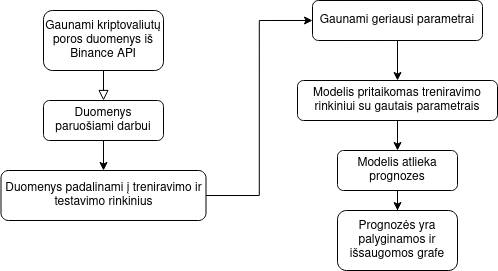
\includegraphics[width=\textwidth]{img/flowchart.png}
  \label{fig:forecast_flowchart}
  \caption{Struktūrinė schema}
\end{figure}

\subsection{Vertinimas}

Vidutinė kvadratinė paklaida (MSE) ir vidutinė absoliučioji procentinė paklaida (MAPE) yra dvi dažniausios metrikos, naudojamos prognozavimo modelių našumui įvertinti.
MSE yra prognozuotų ir faktinių verčių vidutinio skirtumo kvadrato matas, o MAPE yra vidutinio procentinio skirtumo tarp numatytų ir faktinių verčių matas.
Abu šie rodikliai gali būti naudingi lyginant ARIMA ir SARIMA prognozavimo kriptovaliutoms rezultatus.
MSE yra gera metrika norint išmatuoti, kiek prognozės nukrypsta nuo faktinių verčių, mažesnė MSE reikšmė rodo tikslesnį modelį. 
MAPE yra gera metrika prognozavimo paklaidoms procentais matuoti, mažesnė MAPE reikšmė rodo tikslesnį modelį.
Abi šios metrikos gali būti naudojamos vertinant modelių veikimą ir lyginant ARIMA ir SARIMA prognozavimo kriptovaliutoms rezultatus.

% An evaluation of the performance of your models against the actual crypto prices, and a discussion of how well your models were able to predict future prices.
% A schematic or flowchart that visually illustrates the steps of your methodology, which will help your readers understand the process you used.
% A discussion of any evaluation metrics you will be using to assess the performance of your models, such as mean squared error or Akaike information criterion.

\section{Prognozių realizacija}
Šio darbo realizavimo ir rezultatų skyriuje pristatomas metodikos įgyvendinimas ir gauti rezultatai. 
Skyriuje pateikiamos duomenų ir prognozavimo rezultatų vizualizacijos, taip pat kodo fragmentai, demonstruojantys naudojamų modelių įgyvendinimą.
Vizualizacijos suteikia aiškų vaizdą apie modelių veikimą ir prognozių tikslumą. 
Kodo fragmentai suteikia išsamų supratimą apie modelių įgyvendinimą. 
Šioje dalyje taip pat palyginami rezultatai, gauti naudojant ARIMA ir SARIMA modelius, leidžiantys įvertinti modelių veikimą.
\subsection{Modelių realizacija}

Iš pradžių prisijungiama prie testinio tinklo naudojant API ir naudotojo raktus

\begin{python}
  with open(CONFIG_FILE_NAME, 'r') as config_file:
  data = json.load(config_file)
  validate(instance=data, schema=config_schema)
  client = Client(data['api_key'], data['api_secret'], testnet=True)
\end{python}

Tuomet gaunami istoriniai duomenys iš API. Kaip minėta, jog Sausio 4d. įvykio atnaujinimas ir eksperimentiniais tikslais imama duomenys savaitė nuo pradžios į priekį.
tuomet kviečiami funkcija, jog paverstų gautus duomenis į reikalinga struktūrą.

\begin{python}
  klines = client.get_historical_klines(symbol, Client.KLINE_INTERVAL_15MINUTE, end_str='11 Jan, 2023')
  df = binance_klines_to_df(klines)
  model_predict_arima(symbol, df)
  model_predict_arima(symbol, df, seasonal=True)
  
  def binance_klines_to_df(klines):
  klines = np.array(klines)
  df = pd.DataFrame(klines.reshape(-1, 12), dtype=float, columns=('Open Time','Open', 'High', 'Low', 'Close', 'Volume', 'Close time', 'Quote asset volume', 'Number of trades', 'Taker  buy base asset volume', 'Taker buy quote asset volume', 'Ignore'))
  df['Open Time'] = pd.to_datetime(df['Open Time'], unit='ms')
  return df
\end{python}

Turint duomenis kviečiama model\_predict\_arima funckija, kuri pagal seasonal parametrą atlieka ARIMA arba SARIMA modelį.

\begin{python}
  df = df[['Open Time', 'Close']]
  df.set_index('Open Time', inplace=True)
  
  to_row = int(len(df) * 0.9)
  training_data = list(df[0:to_row]['Close'])
  
  if seasonal:
  order, seasonal_order = best_params_arima_seasonal(training_data)
  else:
  order = best_params_arima(training_data)
  seasonal_order = None
  
  testing_data = list(df[to_row:]['Close'])
  model_predictions = []
  for i in range(len(testing_data)):
  model = ARIMA(training_data, order=order, seasonal_order=seasonal_order)
  model_fit = model.fit()
  output = model_fit.forecast(steps=1)
  yhat = output[0]
  model_predictions.append(yhat)
  actual_test_value = testing_data[i]
  training_data.append(actual_test_value)
\end{python}

Pagrindinė kodo dalis atliekanti skaičiavimus
Pasiemama is duomenų tik data ir uždarymo kainą, tuomet duomenys padalijami 90\% apmokymui ir kita dalis prognozavimui. Tuomet modeliui gaunami 
optimalūs parametrai. Po šito inicijuojamas tuščias sąrašas, vadinamas model\_predictions. Kiekvienai iteracijai atliekami šie veiksmus:

\begin{itemize}
  \item sukuria ARIMA modelį turimais duomenimis ir parametrais ir jis yra pritaikomas naudojant fit().
  \item gaunama prognozuojama reikšmė yhat
  \item prie prognozių sąrašo pridedama reikšmė
  \item į turimus duomenis pridedama tikroji reikšmė ir toliau cikliškai apmokamas modelis
\end{itemize}

\subsection{Prognozės}

Šie rezultatai rodo ARIMA ir SARIMA modelių našumą prognozuojant trijų skirtingų simbolių - BTCBUSD, LTCBUSD ir XRPBUSD - kriptovaliutų kainas.
Modelių veikimui įvertinti naudojami MSE (Mean Squared Error) ir MAPE (Mean Absolute Percentage Error). 
MSE matuoja vidutinį skirtumą tarp numatytų ir faktinių verčių kvadratu, o MAPE - vidutinį procentinį skirtumą tarp numatomų ir faktinių verčių. 
Abu šie rodikliai yra svarbūs vertinant modelių tikslumą.

Taikymo rezultatai trims skirtingoms kriptovaliutų poroms: BTCBUSD, LTCBUSD ir XRPBUSD. Grafikuose matosi prognozuota ir tikra kaina laikotarpiu.
BTCBUSD
\begin{figure}[H]
  \centering
  \begin{subfigure}{.5\textwidth}
    \centering
    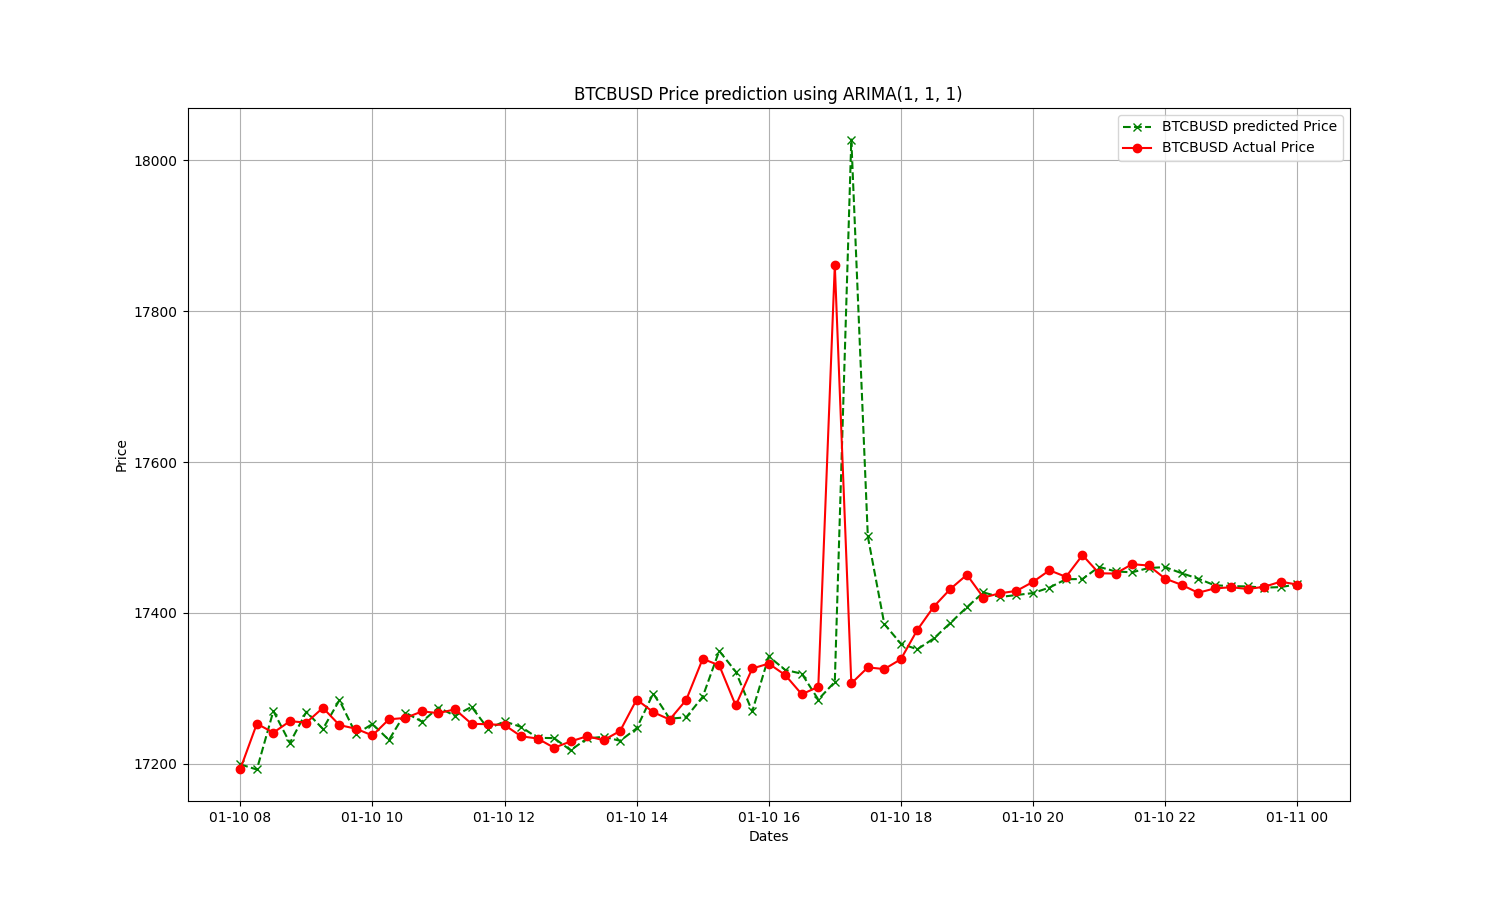
\includegraphics[width=\linewidth]{img/BTCBUSD__ARIMA(1, 1, 1).png}
    \caption{ARIMA modelis}
    \label{fig:btcbusd_arima}
  \end{subfigure}%
  \begin{subfigure}{.5\textwidth}
    \centering
    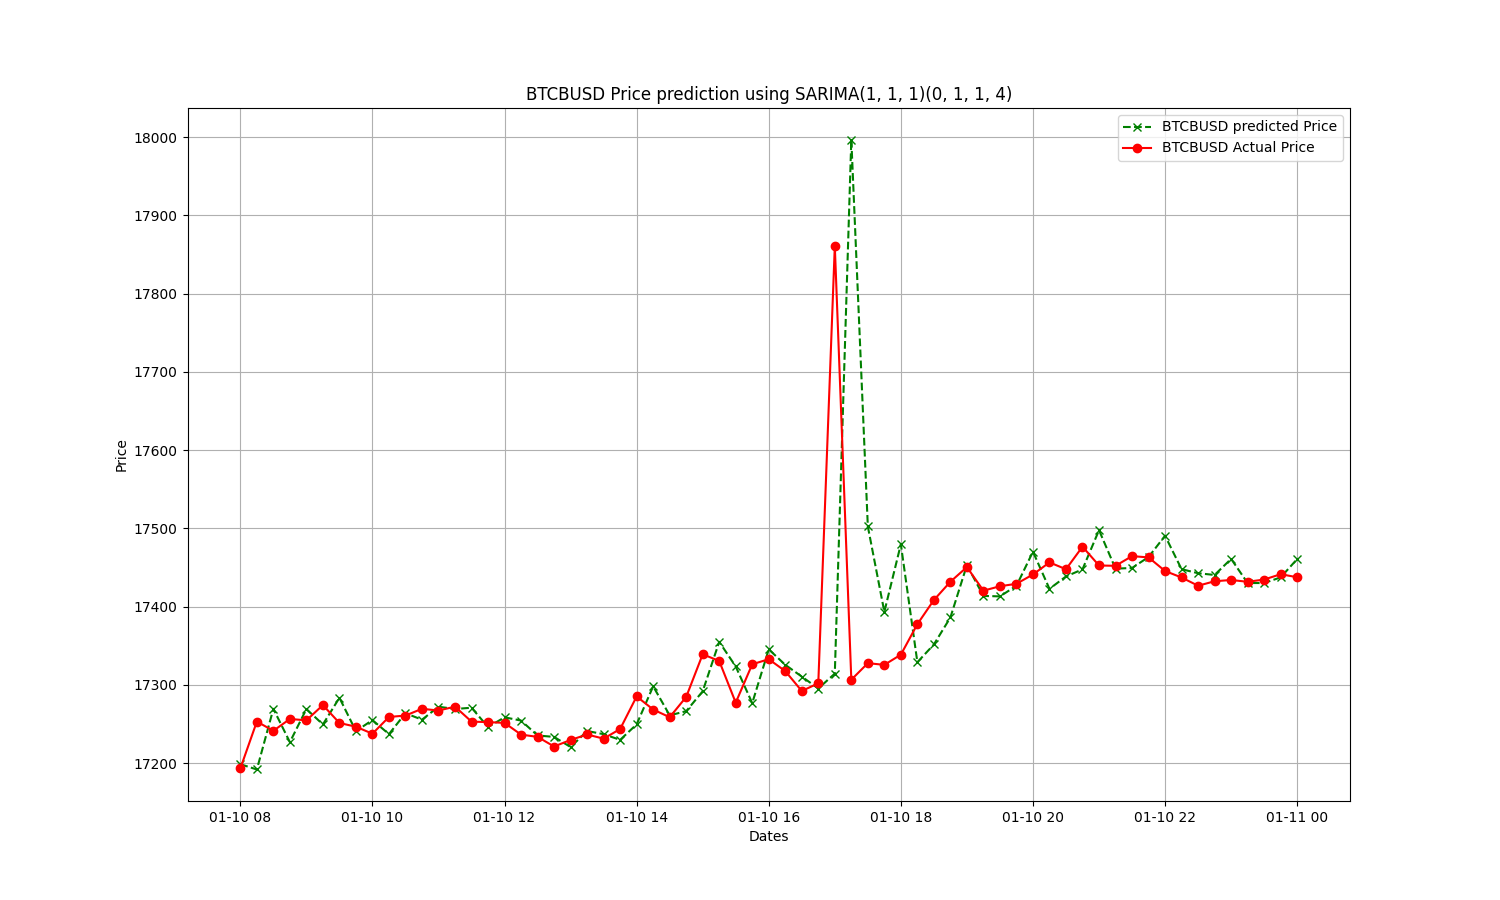
\includegraphics[width=\linewidth]{img/BTCBUSD_seasonal_ARIMA(1, 1, 1)(0, 1, 1, 4).png}
    \caption{SARIMA modelis}
    \label{fig:btcbusd_sarima}
  \end{subfigure}
  \caption{BTCUSD prognozavimas}
  \label{fig:btcbusd}
\end{figure}

LTCBUSD
\begin{figure}[H]
  \centering
  \begin{subfigure}{.5\textwidth}
    \centering
    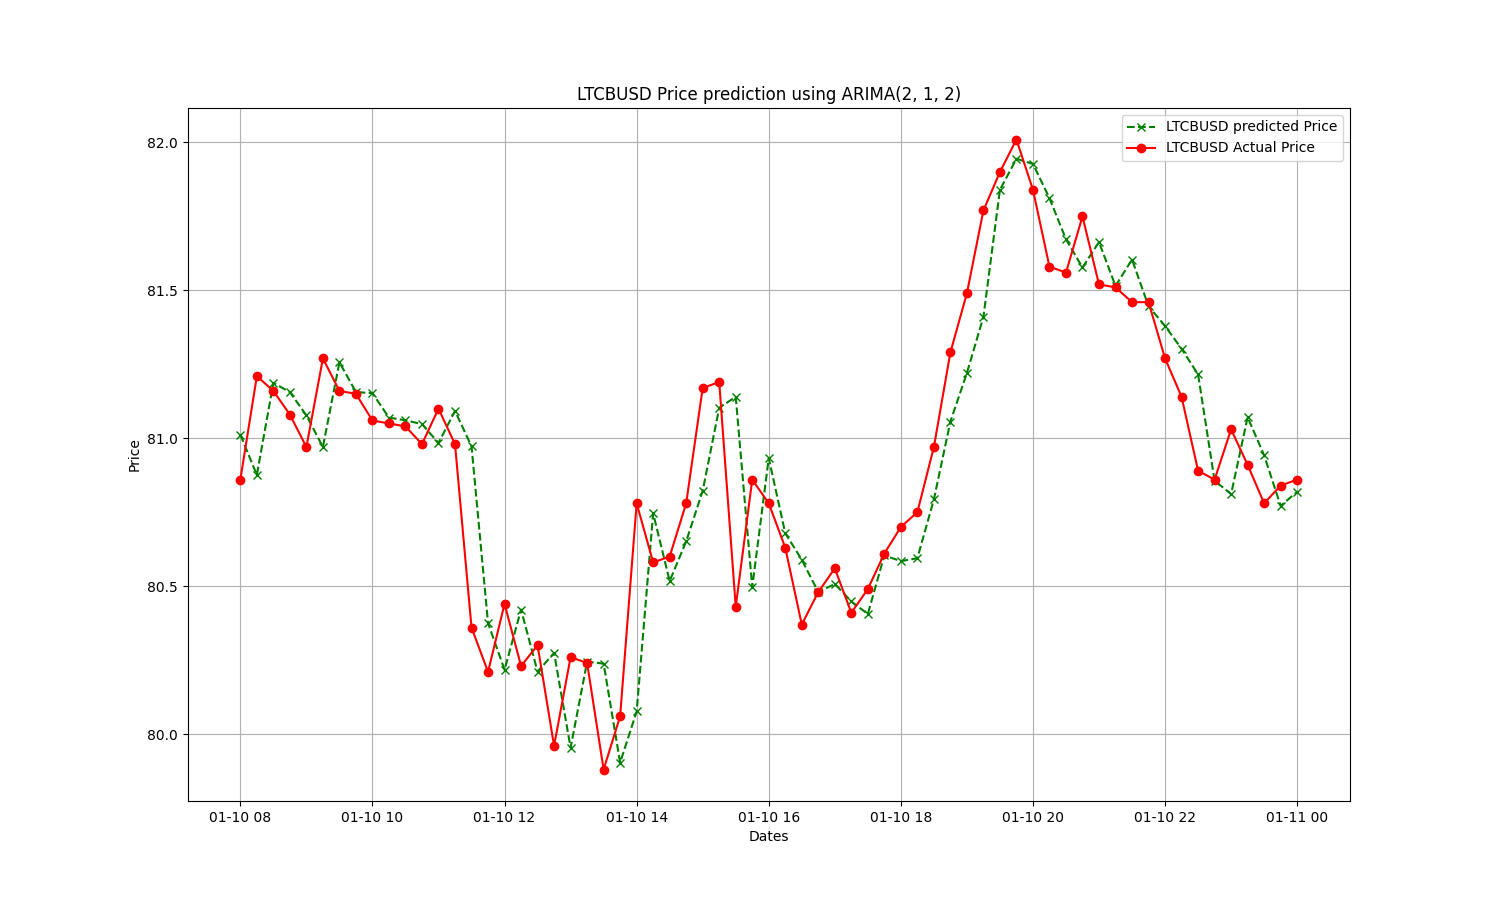
\includegraphics[width=\linewidth]{img/LTCBUSD__ARIMA(2, 1, 2).png}
    \caption{ARIMA modelis}
    \label{fig:ltcbusd_arima}
  \end{subfigure}%
  \begin{subfigure}{.5\textwidth}
    \centering
    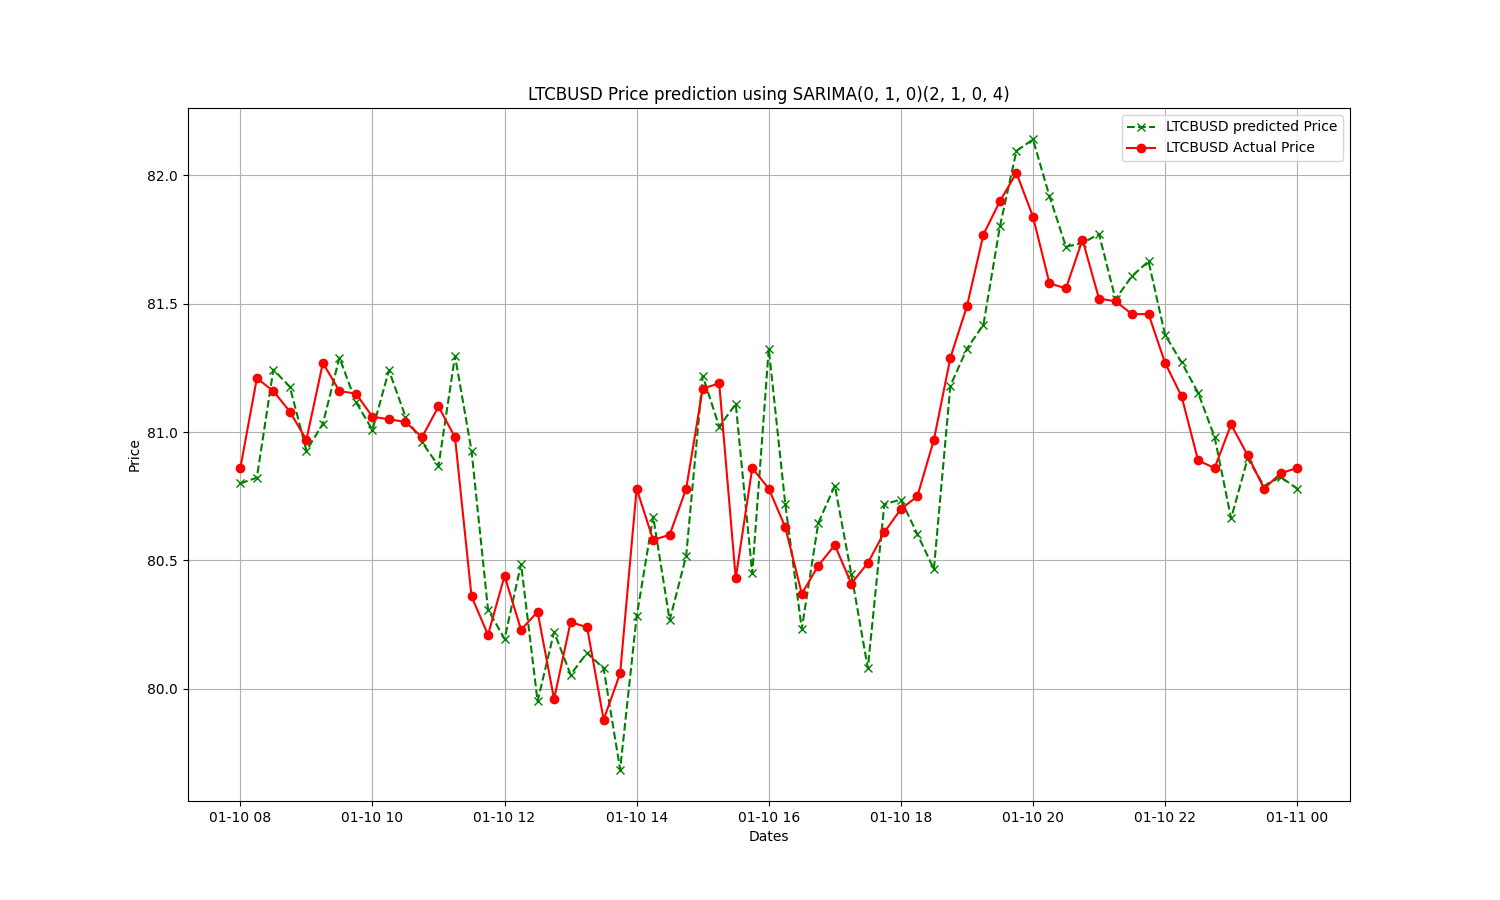
\includegraphics[width=\linewidth]{img/LTCBUSD_seasonal_ARIMA(0, 1, 0)(2, 1, 0, 4).png}
    \caption{SARIMA modelis}
    \label{fig:ltcbusd_sarima}
  \end{subfigure}
  \caption{LTCBUSD prognozavimas}
  \label{fig:ltcbusd}
\end{figure}

XRPBUSD
\begin{figure}[H]
  \centering
  \begin{subfigure}{.5\textwidth}
    \centering
    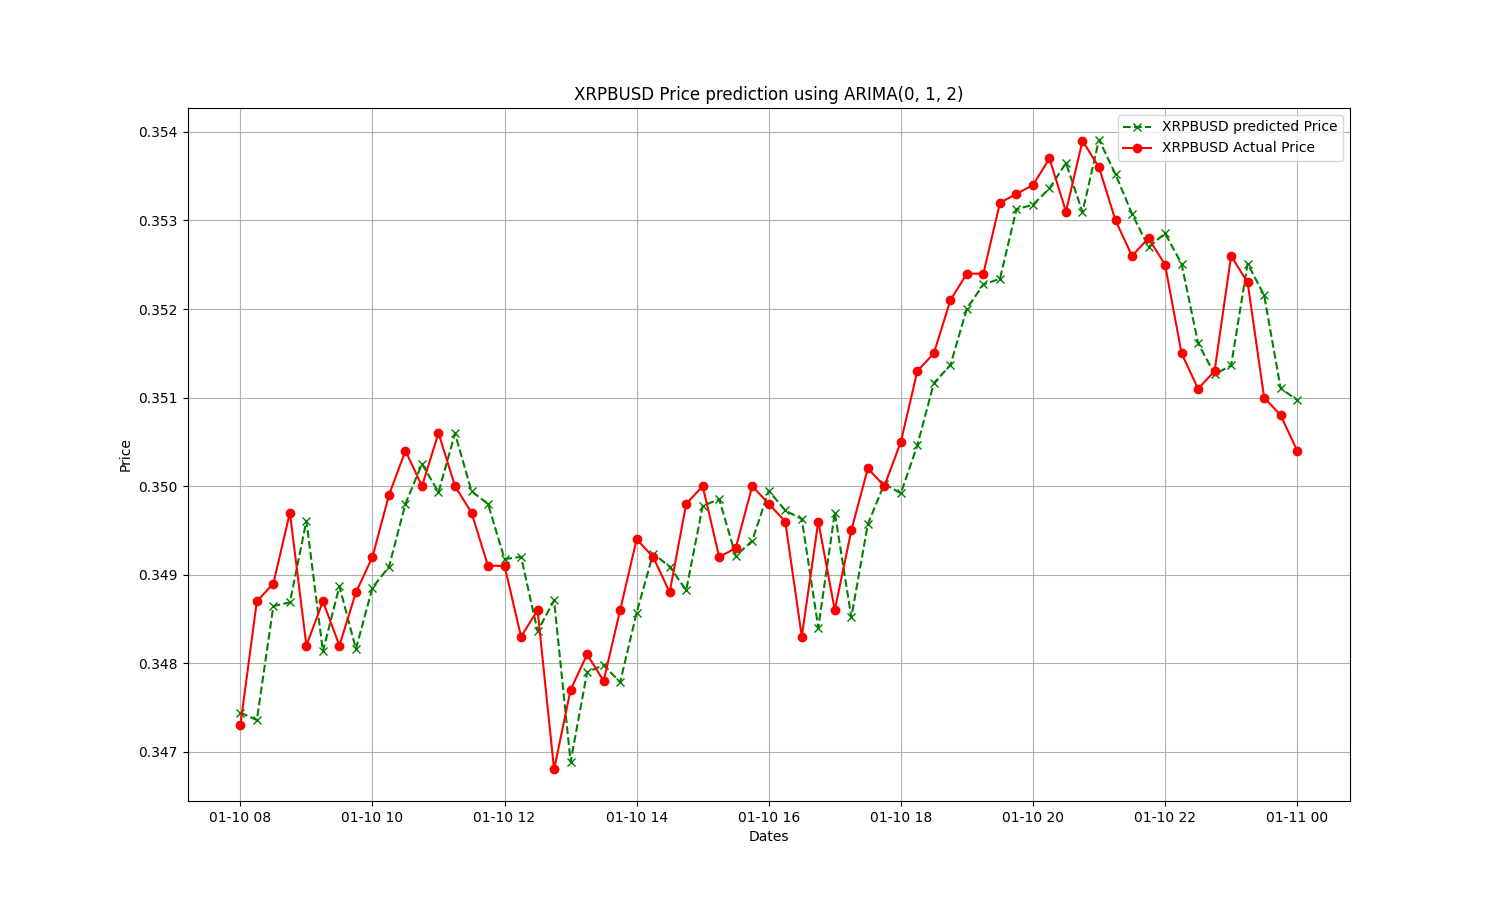
\includegraphics[width=\linewidth]{img/XRPBUSD__ARIMA(0, 1, 2).png}
    \caption{ARIMA modelis}
    \label{fig:xrpbusd_arima}
  \end{subfigure}%
  \begin{subfigure}{.5\textwidth}
    \centering
    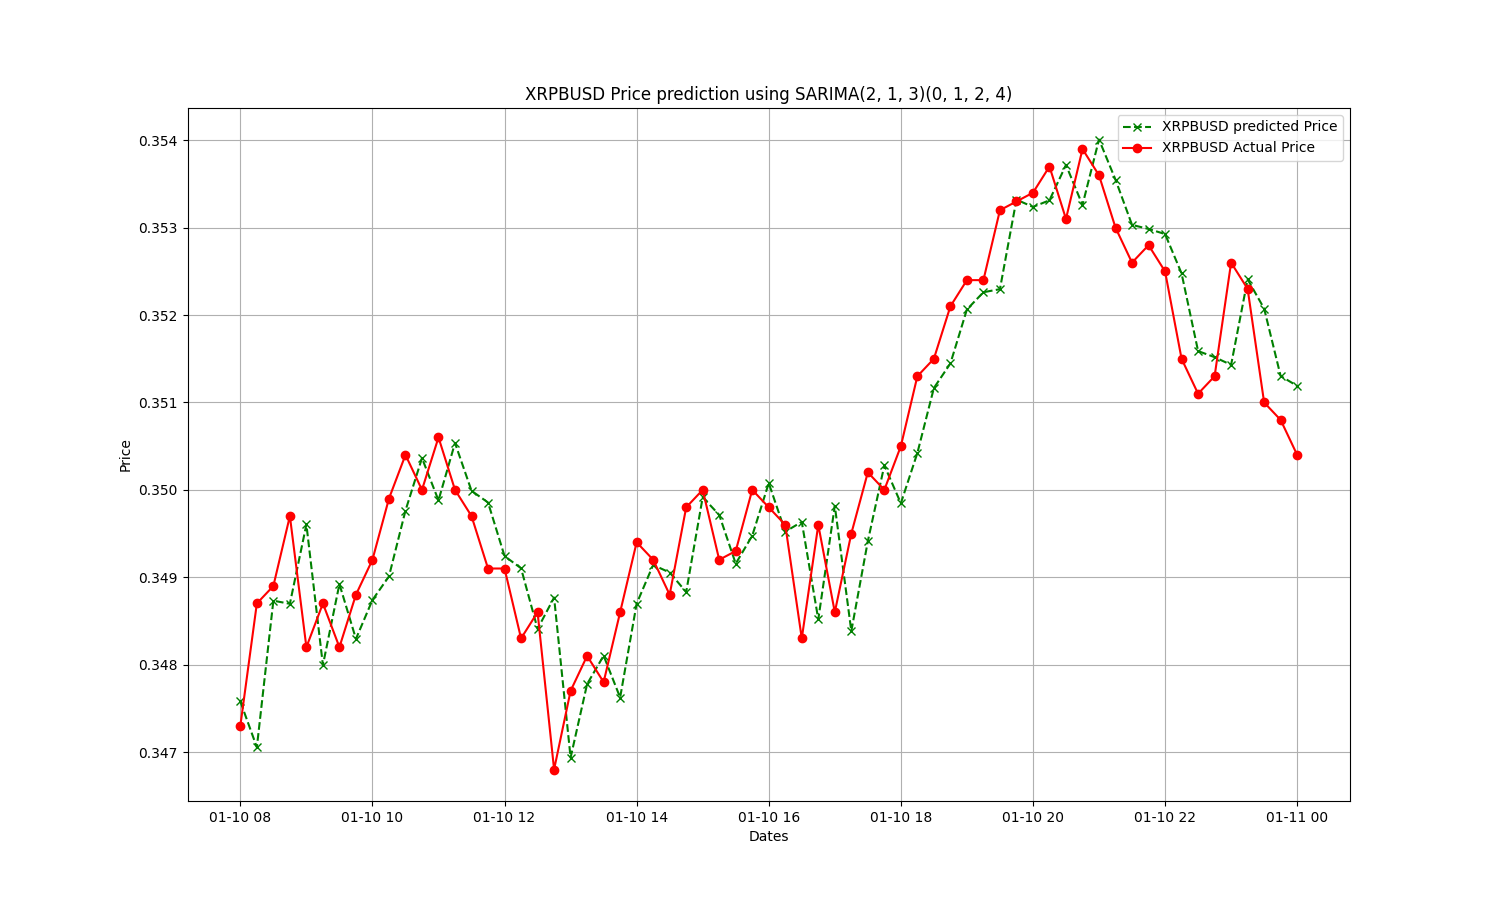
\includegraphics[width=\linewidth]{img/XRPBUSD_seasonal_ARIMA(2, 1, 3)(0, 1, 2, 4).png}
    \caption{SARIMA modelis}
    \label{fig:xrpbusd_sarima}
  \end{subfigure}
  \caption{LTCBUSD prognozavimas}
  \label{fig:xrpbusd}
\end{figure}

\vspace{20pt}

\begin{table}[H]
  \centering
  \begin{tabularx}{\linewidth}{|X|X|X|X|}
    \hline
    Symbol  & Model  & MSE      & MAPE   \\
    \hline
    \hline
    BTCBUSD & ARIMA  & 13702.25 & 0.22\% \\
    \hline
    BTCBUSD & SARIMA & 13349.98 & 0.24\% \\
    \hline
    \hline
    LTCBUSD & ARIMA  & 0.05     & 0.2\%  \\
    \hline
    LTCBUSD & SARIMA & 0.06     & 0.24\% \\
    \hline
    \hline
    XRPBUSD & ARIMA  & 4.92     & 0.16\% \\
    \hline
    XRPBUSD & SARIMA & 5.24     & 0.17\% \\
    \hline
  \end{tabularx}
  \caption{Modelių taikymo rezultatai}
  \label{table:rezultatai}
\end{table}

Iš lentelės matome, kad BTCBUSD poros MSE yra šiek tiek mažesnė SARIMA modeliui nei ARIMA modeliui, tai rodo, kad SARIMA modelis gali šiek tiek geriau atitikti šį duomenų rinkinį, bet MAPE yra šiek tiek mažesnė ARIMA modeliui.

LTCBUSD ir XRPBUSD poroje abiejų modelių MSE ir MAPE yra panašiai žemi, o tai rodo, kad abiejų modelių šių duomenų rinkinių našumas yra panašus. Visų porų MSE ir MAPE yra palyginti žemos, o tai rodo, kad modeliai gerai tinka duomenims, o prognozės yra gana tikslios.

Verta paminėti, kad šie rezultatai yra naudojami konkrečiams duomenų rinkiniui, taigi modeliai gali duoti skirtingus rezultatus kitiems rinkiniams.

\section{Prekybos robotas}
Skyriuje siekiama nuodugniai pažvelgti į sandorių atlikimo metodiką bei įvairių roboto kūrimo strategijų taikytų strategijų rezultatus.
Pagrindinis dėmesys bus skiriamas paaiškinimui, kaip vykdomi sandoriai ir kokie rezultatai gaunami naudojant skirtingus metodus.

\subsection{Metodika}
Robotas yra parašytas naudojamas "python" programavimo kalbą. Yra keli pagrindiniai žingsniai roboto veikime

\begin{enumerate}
  \item Įkeliama konfigūracija ir simbolių duomenys iš failų, duomenys patikranami pagal validacijos schemas ir inicijuojami API prieigos ir klasės kintamieji.
  \item Gaunami istoriniai simbolių "klines" duomenys ir išsaugojami naudojimui.
  \item Skaičiuojama ARIMA prognozes simbolių porų kainoms arba skaičiuojama slankiuosius vidurkius (SMA) simbolių poroms pagal prekybos parametrus.
  \item Siūlomas vartotojui sąveikos su prekybos robotu parinkčių meniu, pvz., likučių, pavedimų, pozicijų, simbolių informacijos spausdinimas ir pavedimų atšaukimas.
  \item Robotas bando atlikti sandorius, jei tenkinamos tam tikros sąlygos, pavyzdžiui, jei trumpasis SMA kerta virš ilgojo SMA, t.y. strategija tenkina sąlygas.
  \item Jeigu įvykdoma transakcija, jį išsaugojama žurnale.
  \item Išsaugo porų duomenis, kai vartotojas išeina iš programos.
\end{enumerate}

Tai yra trumpa ir bendra metodika visais atvejais.
\subsection{Rezultatai}

Toliau robotui sandoriams atlikti pasirinktos šios kriptovaliutų poros 
\begin {itemize}
\item BTC/BUSD
\item LTC/BUSD
\item XRP/BUSD
\item BNB/BTC
\item ETH/BTC
\end {itemize}
Šios poros yra populiarios ir dažnai prekiaujamos tinkle, todėl jomis bus paprasčiau naudotis. 
\subsubsection{Strategijos}
\subsubsubsection{Tendencijos sekimas}

Šiuo atveju vykdoma strategija yra standartinė pirkimo ir laikymo strategija. Robotas naudoja ARIMA, kad sudarytų pasirinktų kriptovaliutų porų kainos prognozes. 
Kai prognozė numato kylančią kainą, robotas įvykdys pirkimo pavedimą, o prognozei numatant mažėjančią kainą robotas vykdys pardavimo pavedimą. 
Šio tipo strategija paremta idėja, kad galima pasipelnyti iš rinkos tendencijų perkant pigiai ir parduodant brangiai.
Robotas naudoja ARIMA, kad analizuotų istorinius kainų duomenis ir prognozuotų būsimus kainų pokyčius, kuriuos jis naudoja priimdamas pirkimo ir pardavimo sprendimus.
Vadovaudamasis šia strategija, robotas siekia pasinaudoti rinkos tendencijomis. 

\begin {itemize}
\item ARIMA prognozuoja kriptovaliutos kainą.
\item Remiantis prognoze, jei modelis numato didėjimo tendenciją, bandoma nusipirkti kriptovaliutą, o jei prognozuoja mažėjimo tendenciją, bandoma kriptovaliutą parduoti.
\item Nuolat stebima kriptovaliutos kainą ir atitinkamai atnaujinamas ARIMA modelis, kad būtų atnaujintos prognozes.
\end{itemize}

Gauti rezultatai taikant šią strategiją

\subsubsubsection{"Mean reversion"}

Mean Reversion yra prekybos strategija, pagrįsta idėja, kad kainos laikui bėgant grįžta į savo vidurkį. 
Tai apima dabartinės kainos palyginimą su istorine vidutine kaina. Sandoris yra sudaromas pagal tai, ar dabartinė kaina yra didesnė ar mažesnė už vidutinę.
Pagal šią strategiją, jei dabartinė kaina yra didesnė už istorinį vidurkį, prekiautojas parduotų turtą, o jei ji yra mažesnė, prekiautojas pirktų. 
Tikslas - pasinaudoti rinkos tendencija grįžti prie vidurkio.

\begin {itemize}
\item Apskaičiuojama kriptovaliutos pastarųjų 5 ir 15 intervalų (15 minučių) paprastą slenkantį vidurkį (SMA).
\item Jei 5 intervalų SMA yra didesnis nei 15 intervalų SMA, bandoma parduoti kriptovaliutą.
\item Jei 5 intervalų SMA yra mažesnis nei 15 intervalų SMA, bandoma pirkti kriptovaliutą.
\item Nuolat stebima kriptovaliutos kaina ir atitinkamai atnaujinami SMA.
\end {itemize}

Strategija grindžiama idėja, kad kai kriptovaliutos kaina nukrypsta nuo vidutinės vertės, ji ilgainiui grįš į vidutinę. Šiuo atveju vidurkį atstoja kainos paprastasis slankusis vidurkis (SMA),
o nuokrypis nuo vidurkio nustatomas lyginant trumpalaikį SMA ir ilgalaikį SMA. Jei trumpalaikis SMA yra didesnis nei ilgalaikis SMA, tada daroma prielaida, kad kaina nukrypsta nuo vidurkio
ir galiausiai grįš, todėl bandoma atlikti pardavimą. Ir atvirkščiai, jei trumpalaikis SMA yra mažesnis už ilgalaikį SMA, tada pateikiamas pirkimo pavedimas, numatant, kad kaina grįš į vidutinę.

\subsubsubsection{"Momentum"}


% Išvadose ir pasiūlymuose, nekartojant atskirų dalių apibendrinimų,
% suformuluojamos svarbiausios darbo išvados, rekomendacijos bei pasiūlymai.
\section{Išvados}
Sukurtas robotas gebantis prekiauti kriptovaliutomis.
\begin{itemize}
  \item atlikta autoregresinių modelių analizė,
  \item parinkta naudoti ARIMA modelį prognozėmis,
  \item sukurtas robotas gebantis prekiauti remantis ARIMA prognozėmis
\end{itemize}

Neišvengiama, jog tokiame trumpame darbe būtų aptartos visos įmanomos sritys ir atvejai, taigi tolimesnei tyrimo eigai pasiūlymas nagrinėti kitus modelius
ir duomenų rinkinius, kad būtų galima palyginti prognozavimo būdus aptartais šiame darbe. Taip pat galima analizuoti alternatyvias strategijas kurias galima
pritaikyti robotui ir jas palyginti. 

\sectionnonum{Sąvokų apibrėžimai}
\textbf{API} - Aplikacijų programavimo sąsaja (angl. Application programming interface), tai sistemos suteikiama sąsaja, kuria galima naudotis norint pasiekti tos sistemos
funckionalumą ar apsikeisti duomenimis.

\textbf{Autoregresinis modelis} - Statistinis modelis yra autoregresinis, jei jis numato būsimas reikšmes pagal praeities reikšmes. Pavyzdžiui, autoregresinis modelis gali
siekti numatyti būsimas akcijų kainas, remiantis ankstesniais rezultatais.

\textbf{Euristinis algoritmas} - euristiniai algoritmai yra tokios intelektualios optimizavimo uždavinių sprendimo priemonės, kuriomis siekiama rasti aukštos
kokybės (bet nebūtinai optimalius) sprendinius per priimtiną laiką. Algoritmas negarantuoja, kad rastas sprendimas bus optimalus. \cite{misevivcius2009euristiniku}

\textbf{Kriptovaliuta} - Kriptovaliuta yra skaitmeninė arba virtuali valiuta, kuri yra apsaugota kriptografija, todėl beveik neįmanoma jos padirbti ar išleisti dvigubai.

\textbf{Kriptovaliutų pora} - Kriptovaliutų pora rinkoje yra naudojama prekiaujant. Kriptovaliutos yra susietos poromis, tad norint nusipirkt BTC valiutos pirmiausia reikia surasti 
galimus keitimo variantus, jei egzistuoja pora BTC/BUSD, galima nusipirkti BTC kriptovaliutos uz turimas BUSD valiutas. Dažnu atveju rinkoje pasidėjus ("FIAT") valiuta
prekybos rinką ją konvertuoją i panašių token valiuta kaip BUSD(us -regulated stablecoin), USDT (usd tether) ar BNB (binance coin)

\textbf{MSE} - Vidutinė kvadratinė paklaida, angl. (Mean squared error)

\textbf{MAPE} - Vidutinė  bsoliučioji paklaida išreikšta procentais, angl. (Mean absolute percentage error)

\printbibliography[heading=bibintoc] % Aprašomi literatūros šaltiniai

\appendix  % Priedai
% Prieduose gali būti pateikiama pagalbinė, ypač darbo autoriaus savarankiškai
% parengta, medžiaga. Savarankiški priedai gali būti pateikiami kompiuterio
% diskelyje ar kompaktiniame diske. Priedai taip pat vadinami ir numeruojami.
% Tekstas su priedais siejamas nuorodomis (pvz.: \ref{img:mlp}).

\end{document}
